\documentclass[11pt]{article}
\usepackage[margin=1in]{geometry}
\usepackage[T1]{fontenc}
\usepackage{lmodern}
\usepackage{microtype}
\usepackage{amsmath,amssymb,amsthm,booktabs,graphicx}
\usepackage[colorlinks=true,linkcolor=blue,urlcolor=blue,citecolor=blue]{hyperref}
\newtheorem{theorem}{Theorem}
\newtheorem{lemma}{Lemma}
\newcommand{\R}{\mathbb R}
\newcommand{\C}{\mathbb C}
\newcommand{\Tr}{\operatorname{Tr}}
\newcommand{\Sp}{\operatorname{Sp}}
\newcommand{\dd}{\,\mathrm d}
\setlength{\parindent}{0pt}
\setlength{\parskip}{0.65em}

\title{The Sixth Nonlinear-Eigenvalue Trace Coefficient\\
\large Radial quadratic cases in dimensions 9 and 11}
\author{Proof packet by \texttt{agent\_lane\_06}}
\date{22 July 2026}

\begin{document}
\maketitle

\textbf{Status.} Candidate partial result, likely valid, subject to human
review.  This settles the first uncomputed coefficient cases singled out in
the source for one positive elliptic polynomial, not for all such
polynomials.

\section{Source problem}

For a positive elliptic polynomial $P$ on $\R^d$, Aboud and Robert study the
quadratic operator pencil
\[
  L(\lambda)=-\Delta+(P(x)-\lambda)^2
\]
and its nonlinear spectrum.  Their semiclassical trace formula has
coefficients $C_{2j}^{(d)}(f)$.  In odd dimensions they prove
$C_{2j}^{(d)}(f)=0$ when $d\geq4j+1$, and conjecture that the next two
coefficients do not vanish: for each $j\geq1$, an admissible $f$ should exist
with
\[
 C_{2j}^{(4j-1)}(f)\ne0,
 \qquad C_{2j}^{(4j-3)}(f)\ne0.
\]
The source verifies $j=1$, treats several $j=2$ cases, and states explicitly
that $d=9,11$ require symbolic or numerical help to compute $C_6^{(d)}$
\cite{AR}.

\begin{figure}[ht]
  \centering
  
\includegraphics[width=\textwidth]{figures/open_conjecture_crop.png}
  \caption{Conjecture (4.25) in the source, PDF page 8.}
\end{figure}

\begin{figure}[ht]
  \centering
  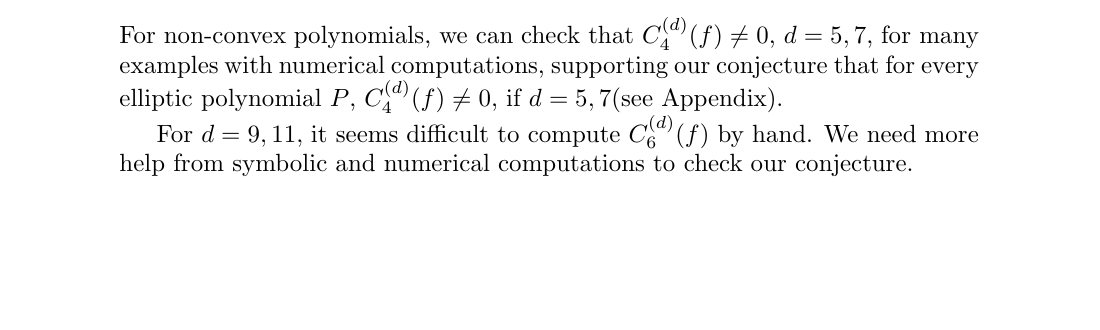
\includegraphics[width=\textwidth]{figures/d9_d11_symbolic_prompt_crop.png}
  \caption{The source's explicit $d=9,11$ symbolic-computation prompt, PDF page 15.}
\end{figure}

\clearpage
\section{Result}

\begin{theorem}\label{thm:main}
Let $P(x)=|x|^2$.  With the source's normalization of the semiclassical trace
coefficients,
\begin{align*}
 C_6^{(9)}\bigl((z+1)^{-15}\bigr)
   &=\frac{212857\pi}{901943132160}>0,\\
 C_6^{(11)}\bigl((z+1)^{-18}\bigr)
   &=\frac{84227\pi}{2727476031651840}>0.
\end{align*}
Consequently the pencil
\[
 -\Delta+(|x|^2-\lambda)^2
\]
has infinitely many nonlinear eigenvalues in dimensions $9$ and $11$.
Writing $N(R)$ for the number in $|\lambda|\leq R$, counted with
multiplicity, for every $\varepsilon>0$ there are positive constants such
that, for all sufficiently large $R$,
\[
 N_{d=9}(R)\geq c_\varepsilon R^{9/2-\varepsilon},
 \qquad
 N_{d=11}(R)\geq c'_\varepsilon R^{15/2-\varepsilon}.
\]
\end{theorem}

\section{Proof intuition}

For the radial quadratic polynomial, every symbol in the Weyl-parametrix
recurrence is invariant under simultaneous rotations of $x$ and $\xi$.
Therefore it depends only on four scalars:
$a=|x|^2$, $b=|\xi|^2$, $c=x\cdot\xi$, and $w=a-z$.  The apparently
high-dimensional recurrence for $K_6$ then becomes ordinary symbolic
differentiation in these four variables.  Each resulting monomial can be
integrated exactly: spherical averaging removes powers of $c$, the $\xi$
radius gives a beta integral, the $z$ contour gives a derivative of $f$, and
the $x$ radius gives a second beta integral.  The final rational multiples of
$\pi$ are positive.

\section{Invariant recurrence}

Put
\[
 a=|x|^2,\quad b=|\xi|^2,\quad c=x\cdot\xi,\quad w=a-z,
 \quad \ell=b+w^2.
\]
For an invariant function $F(a,b,c,w)$, differentiation with respect to $a$
at fixed $z$ is
\[
 D_aF=(\partial_a+\partial_w)F.
\]
Direct differentiation gives
\begin{align*}
 \Delta_xF&=2dD_aF+4aD_a^2F+4cD_a\partial_cF+b\partial_c^2F,\\
 \Delta_\xi F&=2d\partial_bF+4b\partial_b^2F
                 +4c\partial_b\partial_cF+a\partial_c^2F.
\end{align*}
Define
\begin{align*}
 S_2F={}&\frac14\Delta_xF+\frac w2\Delta_\xi F
     +2aF_b+4c^2F_{bb}+4acF_{bc}+a^2F_{cc},\\
 S_4F={}&\frac1{16}\Delta_\xi^2F.
\end{align*}
These are exactly the order-two and order-four contractions in the source's
Weyl recurrence.  Indeed,
\[
 D_x^4\ell=8(\delta_{ij}\delta_{kl}+\delta_{ik}\delta_{jl}
                    +\delta_{il}\delta_{jk}),
\]
which yields the displayed $S_4$; all mixed $x,\xi$ derivatives of $\ell$
vanish.  Since derivatives of $\ell$ of total order above four vanish, the
recurrence through order six is
\begin{align*}
 K_0&=\ell^{-1},\\
 K_2&=-K_0S_2K_0,\\
 K_4&=-K_0(S_2K_2+S_4K_0),\\
 K_6&=-K_0(S_2K_4+S_4K_2).
\end{align*}
As a convention check, the first identity produced by this recurrence is
\[
K_2=\frac{2dw+4a}{\ell^3}
 +\frac{-4wb-8c^2-8aw^2}{\ell^4},
\]
which is precisely the source's displayed $K_2$ formula specialized to
$P(x)=|x|^2$.

\section{Exact integration}

After putting $K_6$ over a common denominator, the exact recurrence gives
\[
 K_6=\frac{N_d(a,b,c,w)}{2\ell^{10}},
\]
where $N_d$ has $33$ monomials for each of $d=9,11$ and only even powers of
$c$.  For a monomial $a^A b^B c^{2k}w^W/\ell^{10}$, spherical averaging and
the radial beta integral give
\begin{align}\label{eq:xi}
\int_{\R^d}\frac{b^Bc^{2k}}{(b+w^2)^{10}}\dd\xi
={}&a^k\frac{(1/2)_k}{(d/2)_k}
 \frac{\pi^{d/2}\Gamma(B+k+d/2)\Gamma(10-B-k-d/2)}
      {\Gamma(d/2)\Gamma(10)}
 (w^2)^{B+k+d/2-10}.
\end{align}
For every monomial occurring in dimensions $9$ and $11$, the second gamma
argument in \eqref{eq:xi} is strictly positive.  Thus every use of
\eqref{eq:xi} is an ordinary convergent integral, not a termwise analytic
regularization.

The source uses the normalized contour integral
$\oint=(2\pi i)^{-1}\int$.  Hence, for $r\geq1$,
\[
 \oint (a-z)^{-r}f(z)\dd z
   =\frac{(-1)^r}{(r-1)!}f^{(r-1)}(a).
\]
Finally,
\[
 \int_{\R^d}a^p(a+1)^{-q}\dd x
 =\frac{\pi^{d/2}\Gamma(p+d/2)\Gamma(q-p-d/2)}
        {\Gamma(d/2)\Gamma(q)}.
\]
Applying these formulas term by term, including the trace prefactor
$-2(2\pi)^{-d}$, gives the following grouped contributions.  Here the row
$(p,r)$ collects all terms proportional before radial integration to
$a^pf^{(r)}(a)$.

\begin{center}
\begin{tabular}{ccc}
\toprule
$d$ & $(p,r)$ & contribution \\
\midrule
9 & $(0,0)$ & $-11951\pi/33822867456$\\
9 & $(1,1)$ & $1802663\pi/789200240640$\\
9 & $(2,2)$ & $-6605027\pi/3156800962560$\\
9 & $(3,3)$ & $7528807\pi/18940805775360$\\
\midrule
11 & $(2,0)$ & $84227\pi/454579338608640$\\
11 & $(3,1)$ & $-84227\pi/545495206330368$\\
\bottomrule
\end{tabular}
\end{center}

Summing the $d=9$ rows and the $d=11$ rows gives the two constants in
Theorem~\ref{thm:main}.

The chosen functions are admissible: because $P$ has degree $m=2$, the source
requires $\mu>3d/2$, and $15>27/2$, $18>33/2$.  The source's trace criterion
therefore implies that the nonlinear spectrum is nonempty; its counting
proposition and scaling corollary in fact give infinitely many eigenvalues and
the exponents
\[
 (d-2j)\frac{m+1}{m}
  =(d-6)\frac32,
\]
which are $9/2$ and $15/2$.  This proves the theorem. \qed

\section{Verification and reproducibility}

The script \texttt{code/verify\_c6\_radial.py} performs the recurrence and all
integrals in exact SymPy arithmetic.  It asserts the specialized source
formula for $K_2$, checks the convergence condition for every monomial, and
asserts both final constants exactly.  The command
\begin{verbatim}
conda run --no-capture-output -n sandbox python code/verify_c6_radial.py
\end{verbatim}
ends with \texttt{All exact assertions passed.}  The complete recorded output
is in \texttt{verification.md}.

\section{Limitations and novelty check}

This proves Conjecture (4.25) only for $j=3$ and the radial quadratic
polynomial in its two critical odd dimensions.  It does not handle arbitrary
positive elliptic $P$, dimensions arising from $j\geq4$, or completeness of
the generalized eigenfunctions.

A bounded novelty search on 22 July 2026 checked the run's four cheap indexes
and exact web/arXiv searches using the source title, the coefficient notation
$C_{2j}^{(4j-1)}$, the phrases ``positive elliptic polynomial'' and
``nonlinear eigenvalue'', and the dimensions $9,11$.  It found the source,
the earlier Helffer--Robert--Wang work, and later numerical work on quadratic
pencils, but no analytic computation of these two coefficients or theorem
implying the displayed result.  Novelty confidence is therefore moderate,
not definitive, because this is a niche literature and notation-based search
can miss differently phrased results.

\section{Human-review recommendation}

Check first the Weyl-product normalization in $S_2,S_4$ and the sign of the
normalized contour residue.  The exact match of $K_2$ with the source is the
main convention audit.  Then rerun the verifier and inspect the two grouped
sums.  If those checks pass, the result is ready to retain as a rigorous
partial solution.

\begin{thebibliography}{9}
\bibitem{AR}
F. Aboud and D. Robert,
\emph{Asymptotic expansion for nonlinear eigenvalue problems},
J. Math. Pures Appl. 93 (2010), 149--162,
arXiv:0903.0919, \url{https://arxiv.org/abs/0903.0919}.
\end{thebibliography}

\end{document}
